\section{The Approach}
\label{sec:framework}
In this section, we first propose a framework to analyze the correlation of heterogeneous time series, and then we introduce how to use hashing method to do fast searching.

\subsection{Change Based Correlation Coefficient}

The Change Based Correlation Coefficient can be calculated following the framework in Fig. \ref{fig:frame}.
Given a time series, first, we extract the change information of the time series. 
In this work, we regard the change information as bit-stream. In the bit-stream, $1$ denotes there is a change in this sub-series, and $0$ if not. We will introduce the change based information in details in the following section.

After obtaining the change information of the time series, we then calculate the Jaccard similarity\cite{han2011data} coefficient between each other.
As we defined before (Section \ref{sec:formulation}), if two time series often change at the same time, they may have correlation with each other. 
So, here, how often denotes the value of the correlation. In other words, how many $1$ do two time series both have. This is directly the Jaccard Distance.
So, the Jaccard similarity between each bit-stream will be the correlation coefficient between these two time series. 

\begin{figure}[t]
\centering
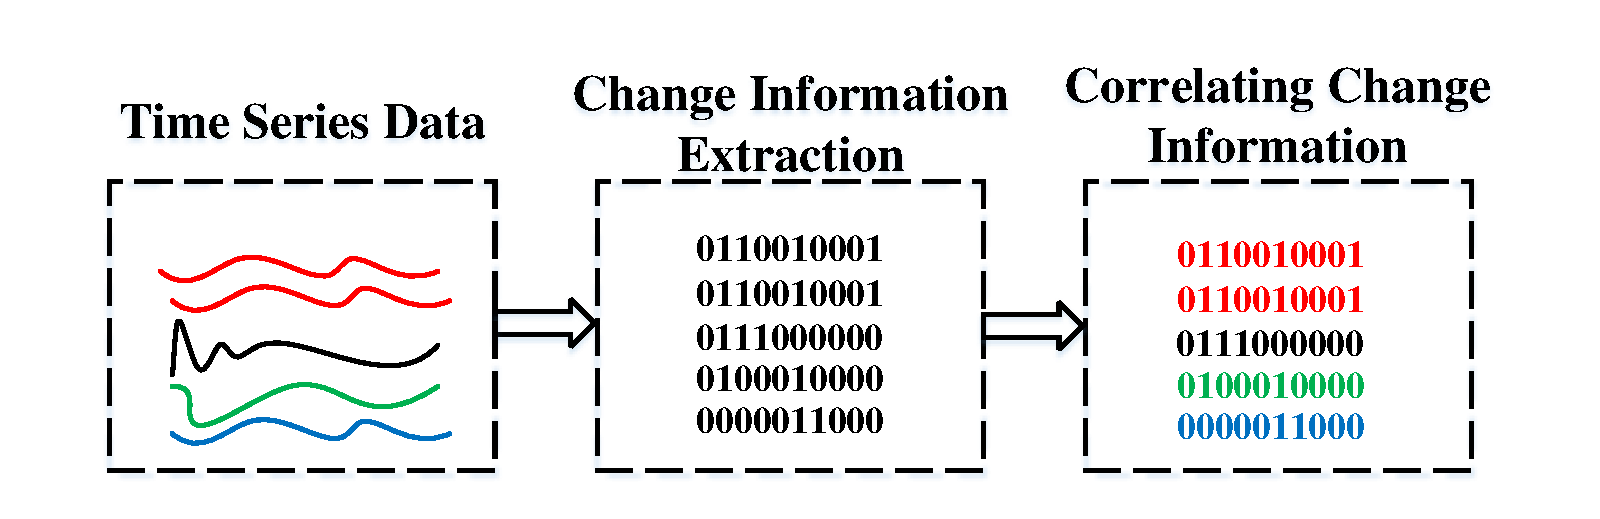
\includegraphics[width=0.5\textwidth]{framework.pdf}
\caption{Overview of the Framework}
\label{fig:frame}
\end{figure}

\subsection{Change Information Extraction}
\label{ChangeCorrelation}

As we introduced in Section.\ref{sec:formulation}, change based correlation corresponds to the change information of the time series. change information of a time series is a time period information, not a time point information. 
As a result, in order to extract the change information of the time series, we need to find the information in small time period of the time series (A sub-series). The idea of extracting the change information is showed in Fig.\ref{fig:ChangeMapping}.

Given a time series $S = (s_1,s_2,...,s_m)$, where $m$ is the number of points in the time series. Given a subs-series length $k$. The change information of the time series $S$ can be represented as a bit-stream:

$B_S = \{b_0,b_1,...,b_n\}$, where each $b_i$ corresponds to a sub-series of length $k$ for the original time series $S$ as showed in 

Given a sub-series $l^j = \{s_i,s_{i+1},s_{i+2},...,s_{i+k-1}\}$, where $w$ is the length of the sub-series. Then the change information of sub-series $l$ is denoted as follow:

\begin{equation}
\label{Equ:ChangeInformation}
b^l = \left\{\begin{matrix}
1 & Have~change~in~l
\\ 
0 & No~change~in~l
\end{matrix}\right.
\end{equation}

\begin{figure}[t]
\centering
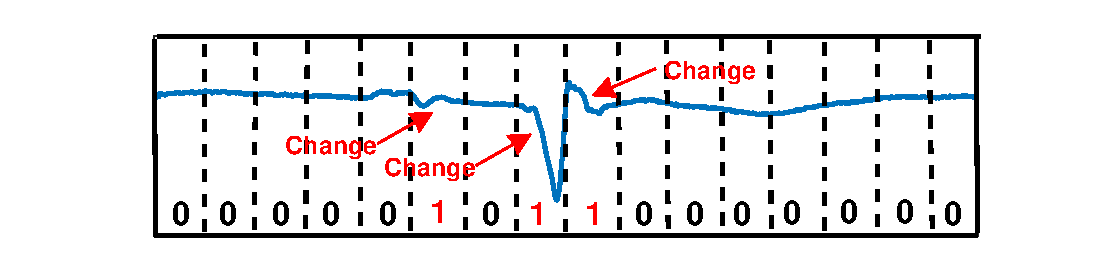
\includegraphics[width=0.5\textwidth]{changeExtraction.eps}
\caption{Change Information Extraction}
\label{fig:ChangeMapping}
\end{figure}

As showed in Equ.\ref{Equ:ChangeInformation}, the change information is the information that whether there's a change in the sub-series. In order to denote whether there's a change in the sub-series, we need to know to to detect change in the sub-series.
Fig.\ref{fig:ChangeMapping} shows how to extract the change information of the time series.

\subsection{Change Detection}
\label{sec:changeDetect}
So,the problem here is:
Given a sub-series 

$l^j = \{s_i,s_{i+1},s_{i+2},...,s_{i+k-1}\}$, 

how to denote whether there is a change or not in this time series.
There are a so many time series change detection methods \cite{liu2013change,chen2013contextual} proposed in the literature. 

In this work, the change detection task here is not find the change points of the time series, instead we only need to denote whether there's a change in the time series. It is pointed out that all the change point detection methods can be used here to detect change information.
In our experiment, we use the the following method to detect change:

We equally divide the time series into two series: 

$l^j_{Front} = \{s_i,s_{i+1},s_{i+2},...,s_{i+(k-1)/2 -1}\}$

and, 

$l^j_{Front} = \{s_{i+(k-1)/2 -1},s_{i+(k-1)/2},...,s_{i+k-1}\}$.

So, regard $l^j_{Front}$ and $l^j_{Rear}$ as two data sampled from two distributions $P_1$ and $P_2$. So, if $P_1$ and $P_2$ are statistically the same, then we can say there's not change between each other. Otherwise, there is a change in this dataset.

Then, the problem here becomes a \textit{Two Sample Problem} \cite{gretton2006kernel}. We use the Two Sample \textit{t}-test \cite{moore2007basic} method to solve this problem:

Here, the $t_{score}$ between $l^j_{Front}$ and $l^j_{Rear}$ can be calculated as:

\begin{equation}
t_{score} = \frac{\overline{l^j_{Front}} - \overline{l^j_{Rear}}}{\sigma_p\sqrt{2/k}}
\end{equation}

where, $\overline{l^j_{Front}}$ and $\overline{l^j_{Front}}$ are the mean values of $l^j_{Front}$ and $l^j_{Front}$. And $\sigma_p$ is as follow:

\begin{equation}
\sigma_p = \frac{(k-1)\sigma_{l^j_{Front}}^2 + (k-1)\sigma_{l^j_{Rear}}^2}{k-1}
\end{equation}

Then, if $t_{score} > \alpha$, we can say that these two samples are from different distributions, and thus there is a change in the sub-series $l^j$.

\subsection{Jaccard Similarity Coefficient}

After obtaining the change information (Bit-stream) of each data, we then use Jacord Similarity Coefficient to calculate the Change Correlation of each time series.

The Jaccard Similarity \cite{han2011data} is defined as follow:
Given two Bit-stream $X$ and $Y$, the Jaccord distance is showed as follow:

\begin{equation}
J(A,B) = \frac{|A \cap B|}{|A \cup B|}
\end{equation}

where, $|A \cap B|$ denotes the number of bit that $X$ and $Y$ both $1$. And $|A \cup B|$ denotes the number of bit that at least $X$ or $Y$ is $1$.
For example, given two bit stream: $X={100111}$, and $Y={001110}$. Then $|A \cap B| = 2$, and $|A \cap B| = 5$, so $J(A,B) = \frac{2}{5} = 0.4$.


\subsection{Speed up Top-k Search using LSH}

In many the real world problems, the scale of time series data often huge \cite{rakthanmanon2012searching}. Mining such huge number of time series is a big challenge for us.

In this work, by taking the advantage of the change based coefficient, we propose to use Locality Sensitive Hashing to do large scale search in time series data.

The change information of a time series is a bit-stream (Section \ref{sec:changeDetect}). We regard it as the hashing code of the original time series.

As ar result, we can directly use LSH (Locality Sensitive Hashing) search algorithm to speed up the searching process. \cite{indyk1998approximate} 

\subsection{Discuss about Sub-series Length w}

In this research, the sub-series length $w$ is a very important parameter.
If the sub-series length $w$ is too short, then the change information can not be captured. 
On the other hand, if the sub-series length $w$ is too long, then there will be too much noise information.

In some cases, the value of $m$ can be selected based on domain knowledge and experiments. In the experiment of this work, all the sub-series length are selected based on the domain knowledge.

However, in most real world situations, there are millions of time series and events, and we do not have enough domain knowledge to pre-select the values of all sub-series lengths. 

In our previous research of Correlating Event with time series \cite{luo2014correlating}, we can auto-select the sub-series length for a time series based on the autocorrelation function \cite{hamilton1994time} of the time series.
Given a time series $S=(s_1,s_2,...,s_n)$, the autocorrelation is showed as follow:

\begin{equation}
R(l) = E(s_i*s_{i-l}).
\end{equation}
where $l$ denotes the lag of the correlation. The autocorrelation function of a time series can be used to represent the energy of signals in the time series with a period of $l$ \cite{hamilton1994time}. Therefore, our length $m$ can be assigned as the value of the first peak to include the significant signal of the time series. For more detail of this selection method, please refer \cite{luo2014correlating}.
